\documentclass{beamer}
\mode<presentation>{
  %   \usetheme{CambridgeUS}      % or try Darmstadt, Madrid, Warsaw, ...
  \usetheme{Frankfurt}
  % \definecolor{mygreen}{cmyk}{0.6,0.168,0.168,0.25}
  % \definecolor{mygreen}{RGB}{84,135,138}

  % \definecolor{myblue}{RGB}{23, 91, 127}
  \definecolor{myblue}{RGB}{24, 71, 160}
  \setbeamercolor{structure}{fg=myblue}
  \usefonttheme{default}
  \setbeamertemplate{navigation symbols}{}
  %\setbeamertemplate[compatibility=false, numbered]{caption}
  \setbeamertemplate{itemize items}[default]
  \setbeamertemplate{enumerate items}[default]
  \defbeamertemplate*{title page}{customized}[1][]{
  \centering
   \begin{beamercolorbox}[rounded=true,shadow=true,leftskip=1cm,colsep*=.75ex]{title}
  \centering
   \usebeamerfont{title}\inserttitle\par
    \end{beamercolorbox}
     \par\medskip\medskip\medskip
     \begin{columns}

     \begin{column}{0.6\textwidth}
     \centering{
          \usebeamerfont{author}\insertauthor\par\medskip\medskip
          \usebeamerfont{institute}\insertinstitute\par\medskip\medskip
          \usebeamerfont{date}\insertdate\par
          \medskip \medskip \medskip
          
\includegraphics[height=0.8cm]{figuras/cnpqLogo.jpg}
    }
    \end{column}
    \begin{column}{0.3\textwidth}
    
\includegraphics[width=\columnwidth]{figuras/brasao_usp_pb}
    \end{column}
    \end{columns}
  }

  \setbeamertemplate{footline}{
    \begin{beamercolorbox}[colsep=1.5pt]{upper separation line foot}
    \end{beamercolorbox}
    \hbox{%
   \begin{beamercolorbox}[wd=0.82\paperwidth, ht=2.5ex, dp=1.125ex, left]{title in head/foot}%
        \usebeamerfont{title in head/foot}\hspace*{2ex}\insertshorttitle
      \end{beamercolorbox}%

      \begin{beamercolorbox}[wd=0.09\paperwidth, ht=2.5ex, dp=1.125ex, center]{title in head/foot}%
        \usebeamerfont{author in head/foot}{\insertshortinstitute }
      \end{beamercolorbox}%
     
      \begin{beamercolorbox}[wd=0.09\paperwidth, ht=2.5ex, dp=1.125ex, right]{title in head/foot}%
        \usebeamerfont{title in head/foot}\insertframenumber/\inserttotalframenumber\hspace*{2ex}
      \end{beamercolorbox}}
    \begin{beamercolorbox}[colsep=1.5pt]{lower separation line foot}
    \end{beamercolorbox}
  }
}

\usepackage{ragged2e}
\usepackage{lipsum}
\usepackage[sort, numbers]{natbib} 
% \usepackage[style=alphabetic]{biblatex}

\makeatletter
\renewcommand{\itemize}[1][]{%
  \beamer@ifempty{#1}{}{\def\beamer@defaultospec{#1}}%
  \ifnum \@itemdepth >2\relax\@toodeep\else
    \advance\@itemdepth\@ne
    \beamer@computepref\@itemdepth% sets \beameritemnestingprefix
    \usebeamerfont{itemize/enumerate \beameritemnestingprefix body}%
    \usebeamercolor[fg]{itemize/enumerate \beameritemnestingprefix body}%
    \usebeamertemplate{itemize/enumerate \beameritemnestingprefix body begin}%
    \list
      {\usebeamertemplate{itemize \beameritemnestingprefix item}}
      {\def\makelabel##1{%
          {%
            \hss\llap{{%
                \usebeamerfont*{itemize \beameritemnestingprefix item}%
                \usebeamercolor[fg]{itemize \beameritemnestingprefix item}##1}}%
          }%
        }%
      }
  \fi%
  \beamer@cramped%
  \justifying% NEW
  %\raggedright% ORIGINAL
  \beamer@firstlineitemizeunskip%
}
\makeatother

\useoutertheme[subsection=false]{miniframes}
\usepackage{etoolbox}
\makeatletter
\patchcmd{\slideentry}{\advance\beamer@xpos by1\relax}{}{}{}
\def\beamer@subsectionentry#1#2#3#4#5{\advance\beamer@xpos by1\relax}%
\makeatother

\usepackage[compatibility=false]{caption}
\usepackage{subcaption}
\usepackage[brazil]{babel}
\usepackage[utf8x]{inputenc}
\usepackage{setspace}
\usepackage{ragged2e}
\usepackage{graphicx}
\usepackage{amsmath,amsfonts,amssymb}
\usepackage{xcolor}
\usepackage{url}
\usepackage{array}
\usepackage{gensymb}
\usepackage{multicol}
\usepackage[loadonly]{enumitem}
\newlist{arrowlist}{itemize}{1}
\setlist[arrowlist]{label=$\Rightarrow$}
\usepackage{listings}
\newcommand{\fonte}[1]{\caption*{Fonte: #1}}
\newcommand{\fonteminha}{\caption*{Fonte: Elaborado pelo autor.}}

\title[\textbf{Geração de imagens artificiais e extração de características latentes aplicadas à classificação de imagens}]{\textbf{Geração de imagens artificiais e extração de características latentes aplicadas à classificação de imagens}}
\author{Gabriela Salvador Thumé \\ \vspace{4pt}
        \tiny Orientador: Prof. Dr. Moacir Pereira Ponti Junior}
\institute[ICMC/USP]{Instituto de Ciências Matemáticas e de Computação \\
Universidade de São Paulo \\ }
\date{27 de março de 2015}
%%%%%%%%%%%%%%%%%%%%%%%%%%%%%%%%%%%%%%%%%%%%%%%%%%%%%%%%%%%%%%%%%%%%%%%%%%%%%%%
\begin{document}
\setbeamercovered{transparent}
\begin{frame}[plain]
  \maketitle
\end{frame}
%%%%%%%%%%%%%%%%%%%%%%%%%%%%%%%%%%%%%%%%%%%%%%%%%%%%%%%%%%%%%%%%%%%%%%%%%%%%%%%
\begin{frame}[noframenumbering]{Estrutura da Apresentação}
\setstretch{1.2}
\begin{multicols}{2}
  \tableofcontents
\end{multicols}
\end{frame}
\section{Introdução}
%%%%%%%%%%%%%%%%%%%%%%%%%%%%%%%%%%%%%%%%%%%%%%%%%%%%%%%%%%%%%%%%%%%%%%%%%%%%%%%
\AtBeginSection[]{
\begin{frame}<beamer>[noframenumbering]{Estrutura da Apresentação}
\setstretch{1.2}
\begin{multicols}{2}
\tableofcontents[currentsection, sectionstyle=show/shaded,
]
% \tableofcontents[currentsection,currentsubsection, hideothersubsections, 
%     sectionstyle=show/shaded,
% ]
\end{multicols}
\end{frame}
}
%%%%%%%%%%%%%%%%%%%%%%%%%%%%%%%%%%%%%%%%%%%%%%%%%%%%%%%%%%%%%%%%%%%%%%%%%%%%%%%
\begin{frame}{Introdução}
\setstretch{1.2}
\setlength\leftmargini{0em}
\justifying
\begin{itemize}
\item Classificação de imagens;
\pause
\item Extração de características;
\pause
\item Algoritmos de aprendizado de máquina: modelo de representação;
\item Generalização permite classificar novos exemplos;
\pause
\item Características que dificultam a diferenciação entre as classes;
\item Encontrar as características que melhor discriminam as classes.
\end{itemize}
\end{frame}
%-----------------------------------------------------------------------------
\subsection{Motivação}
\begin{frame}[plain]{Motivação}
\begin{figure}
    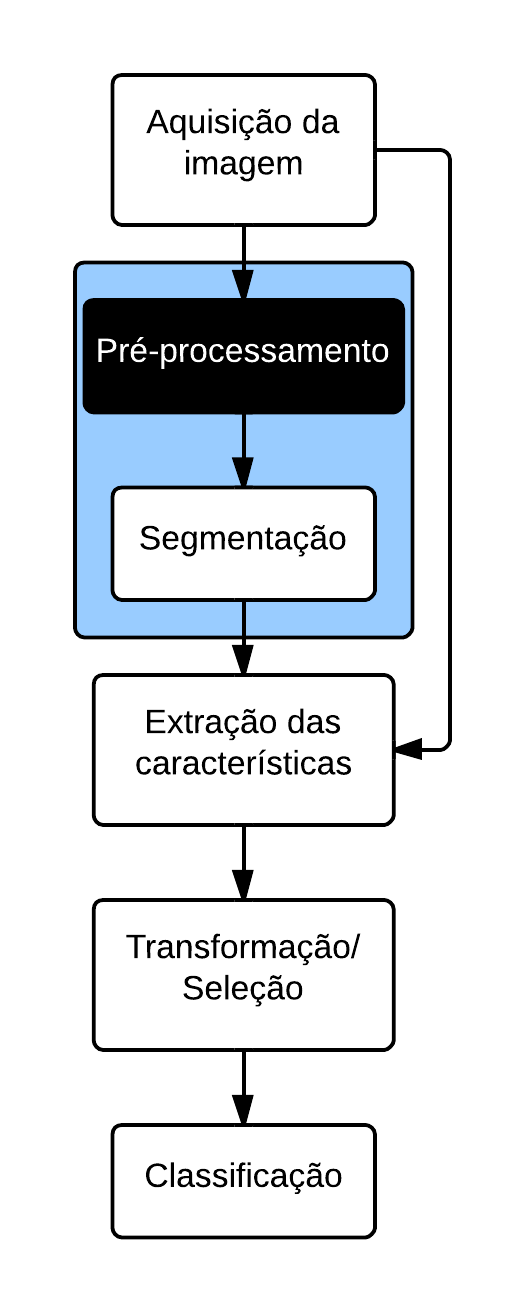
\includegraphics[height=0.9\textheight]{figuras/flow.png}
    \caption{Etapas canônicas do reconhecimento de padrões.}
\end{figure}
\end{frame}
%-----------------------------------------------------------------------------
\begin{frame}{Motivação}
\setstretch{1.2}
\setlength\leftmargini{0em}
\justifying
\begin{itemize}
\item Maior esforço ao operar no espaço de características já obtidas;
\item Transformações do espaço ou sistemas complexos de classificação para lidar com as deficiências das características extraídas;
\item Características que podem ser exploradas além dos métodos clássicos;
\item Investigar métodos de processamento e preparação de imagens antes da extração.
\end{itemize}
\end{frame}
%-----------------------------------------------------------------------------
\begin{frame}{Motivação - Características Latentes}

\renewcommand{\tabcolsep}{0.0cm}
\begin{figure}[htbp]
 \begin{center}
\begin{subfigure}{.15\textwidth}
  \centering
  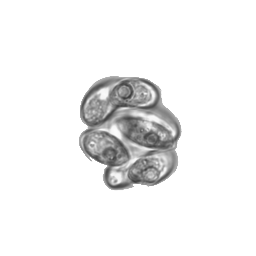
\includegraphics[width=\linewidth]{\detokenize{figuras/alga_05b.png}}
  \caption{}
\end{subfigure}
\begin{subfigure}{.15\textwidth}
  \centering
  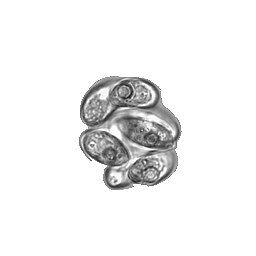
\includegraphics[width=\linewidth]{\detokenize{figuras/alga_05c.png}}
  \caption{}
\end{subfigure}
\begin{subfigure}{.15\textwidth}
  \centering
    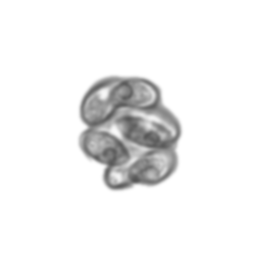
\includegraphics[width=\linewidth]{\detokenize{figuras/alga_05d.png}}
  \caption{}
\end{subfigure}
\begin{subfigure}{.15\textwidth}
  \centering
  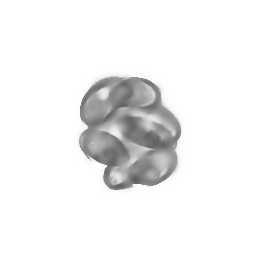
\includegraphics[width=\linewidth]{\detokenize{figuras/alga_05e.png}}
  \caption{}
\end{subfigure}
\\
\begin{subfigure}{.15\textwidth}
  \centering
  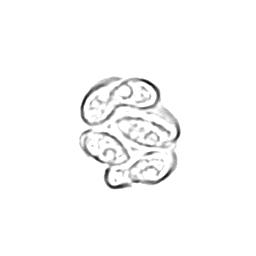
\includegraphics[width=\linewidth]{\detokenize{figuras/alga_05ba.png}}
  \caption{}
\end{subfigure}
\begin{subfigure}{.15\textwidth}
  \centering
  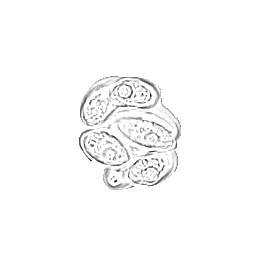
\includegraphics[width=\linewidth]{\detokenize{figuras/alga_05ca.png}}
  \caption{}
\end{subfigure}
\begin{subfigure}{.15\textwidth}
  \centering
  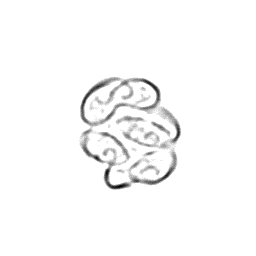
\includegraphics[width=\linewidth]{\detokenize{figuras/alga_05da.png}}
  \caption{}
\end{subfigure}
\begin{subfigure}{.15\textwidth}
  \centering
  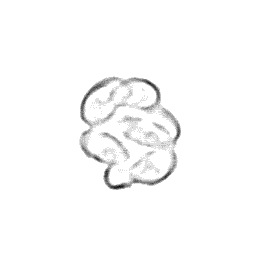
\includegraphics[width=\linewidth]{\detokenize{figuras/alga_05ea.png}}
  \caption{}
\end{subfigure}
\\
\begin{subfigure}{.15\textwidth}
  \centering
  
\includegraphics[width=\linewidth]{\detokenize{figuras/alga_05bb.png}}
  \caption{}
\end{subfigure}
\begin{subfigure}{.15\textwidth}
  \centering
  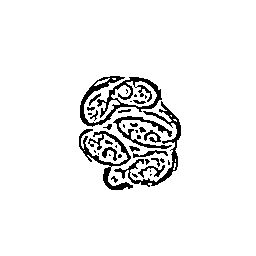
\includegraphics[width=\linewidth]{\detokenize{figuras/alga_05cb.png}}
  \caption{}
\end{subfigure}
\begin{subfigure}{.15\textwidth}
  \centering
  
\includegraphics[width=\linewidth]{\detokenize{figuras/alga_05db.png}}
  \caption{}
\end{subfigure}
\begin{subfigure}{.15\textwidth}
  \centering
  
\includegraphics[width=\linewidth]{\detokenize{figuras/alga_05eb.png}}
  \caption{}
\end{subfigure}
  \caption{Características latentes de algas verdes.}
%{Características latentes de algas verdes. A primeira imagem (a) é uma imagem original segmentada de alga. As próximas colunas são imagens resultantes da deconvolução da imagem (coluna 2), filtragem Gaussiana (coluna 3) e filtragem Gaussiana seletiva (coluna 4). A primeira linha mostra versões diferentes de imagens de algas, a segunda linha exibe imagens resultantes da diferença de Gaussianas, e a terceira linha demonstra imagens binárias obtidas por limiarização das imagens contidas na segunda linha). \textit{Fonte:~Elaborado pelo autor.}}
 \end{center}
\end{figure}
\renewcommand{\tabcolsep}{0.25cm}
\end{frame}
%-----------------------------------------------------------------------------
\begin{frame}{Motivação - Características Latentes}
\setlength\leftmargini{0em}
\justifying
\setstretch{1.2}
\begin{itemize}
\item Justificado o uso de métodos de processamento e preparação de imagens antes da extração;
\item Podem revelar características latentes, não visíveis nas imagens originais;
\item Foco: \emph{realçar características que possam melhor descrever certas classes, utilizando algoritmos sobre as imagens originais.}
\end{itemize}
\end{frame}
%-----------------------------------------------------------------------------
\begin{frame}{Motivação}
\setlength\leftmargini{0em}
\justifying
 \setstretch{1.2}
  \begin{itemize}
\justifying
    % \item Grupo de pesquisa em Visualização, Imagens e Computação Gráfica (VICG)
    % \only<1>{
    %   \begin{itemize}
    %       \item Visualização de informação com projeções multidimensionais e árvores;
    %       \item Extração e classificação de imagens.
    %   \end{itemize}
    % }
    \item 98\% de acurácia após aquisição, pré-processamento e segmentação (Rocha et al., 2010); % frutas
    \item Quantização pode impactar a classificação (Kanan e Cottrell, 2012);
    \item Quantização permite obter vetores de características mais compactos e com maior capacidade de discriminação entre classes (Ponti et al., 2014);
    \item[]  {Continuação: analisar redes que aprendem quais operações geram essas características.}
  \end{itemize}
\end{frame}
%-----------------------------------------------------------------------------
\begin{frame}{Motivação - Desbalanceamento de classes}
\setlength\leftmargini{0em}
\justifying
% \setstretch{1.2}
  \begin{itemize}
    \item Diferença entre o número de exemplos disponíveis;
    \item Imagens representam eventos importantes mas menos frequentes;
    \item Obstáculo, métodos de transformação do espaço e de 
    classificação assumem que a base está balanceada;
    \item Foco: \emph{geração de imagens artificiais a partir do realce de características das imagens da classe minoritária.}
  \end{itemize}
  \begin{figure}[htbp]
 \begin{center}
   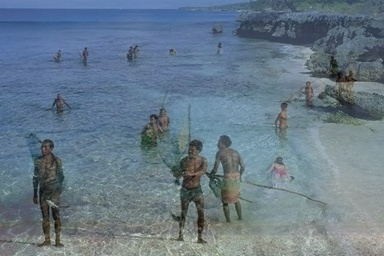
\includegraphics[width=.4\linewidth]{figuras/imagemgerada.jpg}
 \caption{Imagem artificialmente gerada.}
 \end{center}
\end{figure}

\end{frame}
%-----------------------------------------------------------------------------
% \section{Proposta}
\begin{frame}{Proposta da Pesquisa}
 \setstretch{2}
\begin{block}{}
\justifying
    Melhorar a classificação de imagens, utilizando métodos de processamento com foco na \textbf{extração de características latentes} e no \textbf{rebalanceamento de classes.}
\end{block}
\end{frame}
%-----------------------------------------------------------------------------
\subsection{Hipóteses e Objetivos}
\setstretch{1.2}
\setlength\leftmargini{1em}
\justifying
 \begin{frame}{Hipóteses}
  \begin{block}{Métodos de pré-processamento}
    \justifying
    \begin{itemize}
      \item Extrair características latentes que aumentem a variância entre as classes, sem aumentar a variância intra-classe;
      \item Melhorar a classificação.
    \end{itemize}
  \end{block}
  \begin{block}{Geração de imagens artificiais}
    \justifying
    \begin{itemize}
      \item Balancear as classes;
      \item Melhorar a acurácia, versus geração de exemplos artificiais no espaço de atributos.
    \end{itemize}
  \end{block}
\end{frame}
%%%%%%%%%%%%%%%%%%%%%%%%%%%%%%%%%%%%%%%%%%%%%%%%%%%%%%%%%%%%%%%%%%%%%%%%%%%%%%%
\begin{frame}{Objetivo Geral}
\setstretch{1.2}
\setlength\leftmargini{1em}
\justifying
  \begin{block}{}
  \justifying
  \emph{Investigar os métodos de pré-processamento para preparar uma coleção de imagens para a extração de características.}

  \vspace{5mm}
  Espera-se obter características latentes e balancear o número de instâncias de diferentes classes.
  \end{block}
\end{frame}
%-----------------------------------------------------------------------------
\begin{frame}{Objetivos Específicos}
% \setstretch{1.2}
\setlength\leftmargini{1em}
\justifying
    \begin{itemize}
      \item Analisar: 
        \begin{itemize}
          \item impacto de métodos canônicos na classificação;
          \item aprendizado de bases bem discriminadas por redes de convolução.
        \end{itemize}
      \item Tornar as características latentes visíveis;% com o auxílio dos métodos canônicos e CNN;
      \item Gerar imagens artificiais. 
      \pause
        \begin{itemize}
          \item Resultados preliminares;
          % \item Estudo das características latentes encontradas no treinamento da classe minoritária de uma rede de convolução;
          \item Matriz de características aprendida por uma máquina de Boltzmann restrita para verificar a relevância das imagens geradas e as imagens originais.
        \end{itemize}
    \end{itemize}
\end{frame}
%-----------------------------------------------------------------------------
\begin{frame}{Proposta}
\begin{figure}
    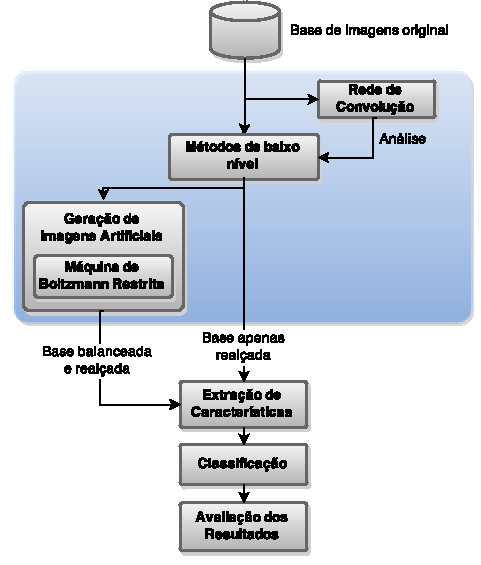
\includegraphics[height=0.75\textheight]{figuras/geral.pdf}
    \caption{Estrutura geral desta pesquisa.}
\end{figure}
\end{frame}
%-----------------------------------------------------------------------------
\section{Contextualização}
\subsection{Pré-processamento}
\begin{frame}{Pré-processamento de Imagens}
\begin{figure}
    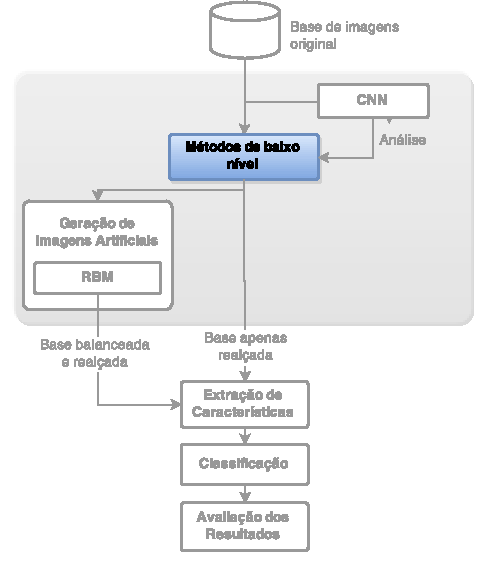
\includegraphics[height=0.75\textheight]{figuras/geral_metodos.pdf}
\end{figure}
\end{frame}
%-----------------------------------------------------------------------------
\begin{frame}{Pré-processamento de Imagens}
\begin{figure}[htbp]
 \begin{center}
   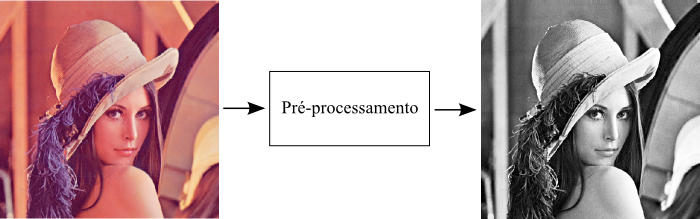
\includegraphics[width=1\linewidth]{figuras/preprocessamento.png}
 \caption{Borramento, realce e de equalização de histograma.}
 \end{center}
\end{figure}
\end{frame}
%-----------------------------------------------------------------------------
\begin{frame}{Pré-processamento de Imagens - Convolução}
\setlength\leftmargini{0em}
\justifying
\setstretch{1.2}
\begin{itemize}
    \item Percorre a imagem com um filtro espacial rotacionado em $180\degree$; \\
    \item Cria cada novo pixel com as mesmas coordenadas do centro da vizinhança contendo o valor resultante da filtragem.
\end{itemize}
\begin{figure}[htbp]
 \begin{center}
   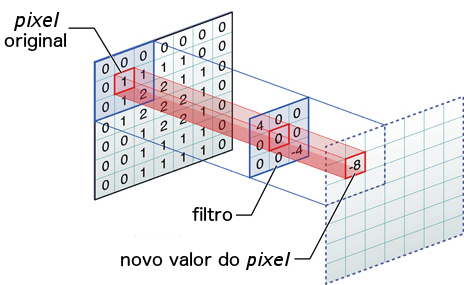
\includegraphics[width=.5\linewidth]{figuras/convolucao.png}
 \caption{Convolução com filtro previamente rotacionado.}
 \end{center}
\end{figure}
\end{frame}
%-----------------------------------------------------------------------------
\begin{frame}{Pré-processamento de Imagens - Convolução}
  \begin{figure}[!hbpt]
    \begin{center}
    \begin{subfigure}{.4\textwidth}
    \centering
      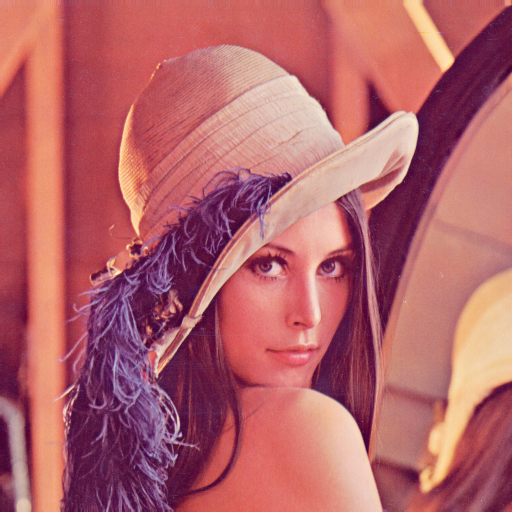
\includegraphics[width=\linewidth]{\detokenize{figuras/original.png}}
      \caption{Original}
    \end{subfigure}
    \hspace{0.1\textwidth}
    \begin{subfigure}{.4\textwidth}
    \centering
      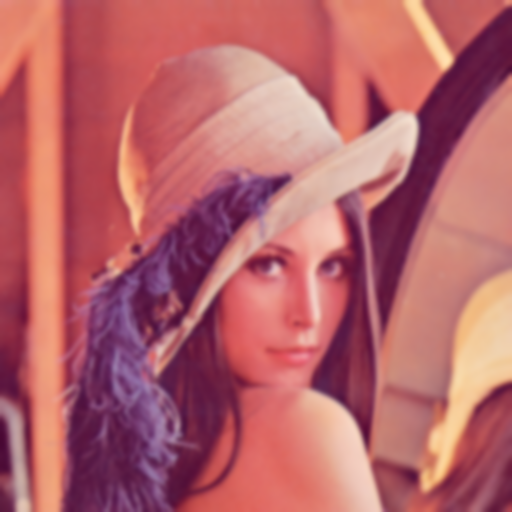
\includegraphics[width=\linewidth]{\detokenize{figuras/blur.png}}
      \caption{Filtragem Gaussiana}
    \end{subfigure}
    \end{center}
    \end{figure}
\end{frame}
%-----------------------------------------------------------------------------
\begin{frame}{Pré-processamento de Imagens - Realce}
\begin{figure}[!htbp]
 \begin{center}
\begin{subfigure}{.4\textwidth}
  \centering
  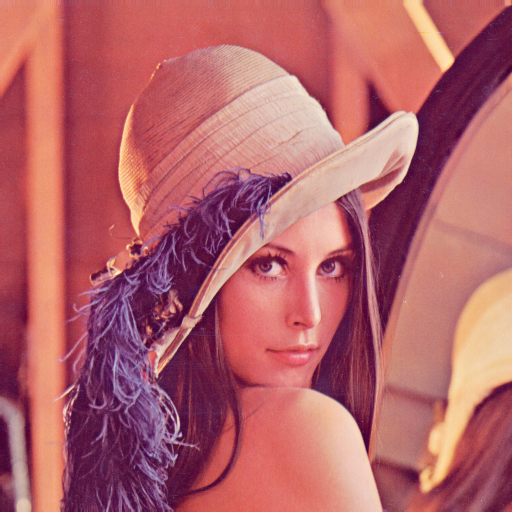
\includegraphics[width=\linewidth]{\detokenize{figuras/original.png}}
  \caption{Original}
\end{subfigure}
\hspace{0.1\textwidth}
\begin{subfigure}{.4\textwidth}
  \centering
  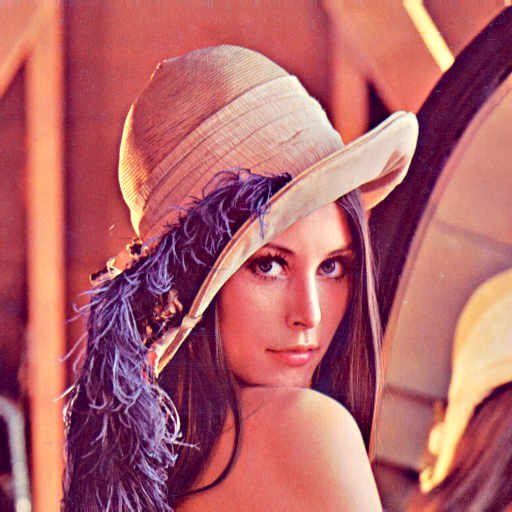
\includegraphics[width=\linewidth]{\detokenize{figuras/unsharpmask.png}}
  \caption{\textit{Unsharp masking}}
\end{subfigure}
 \end{center}
\end{figure}
\end{frame}
%-----------------------------------------------------------------------------
\begin{frame}{Pré-processamento de Imagens - Quantização}
\begin{figure}
 \begin{center}
\begin{subfigure}{.3\textwidth}
  \centering
  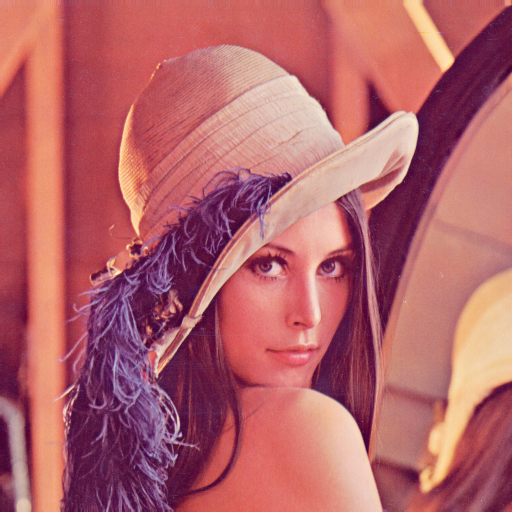
\includegraphics[width=\linewidth]{\detokenize{figuras/original.png}}
  \caption{Original}
\end{subfigure}
\begin{subfigure}{.3\textwidth}
  \centering
  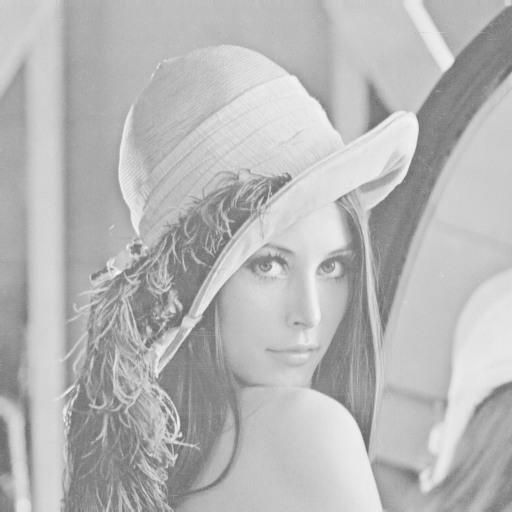
\includegraphics[width=\linewidth]{\detokenize{figuras/intensity.png}}
  \caption{Intensidade}
\end{subfigure}
\begin{subfigure}{.3\textwidth}
  \centering
  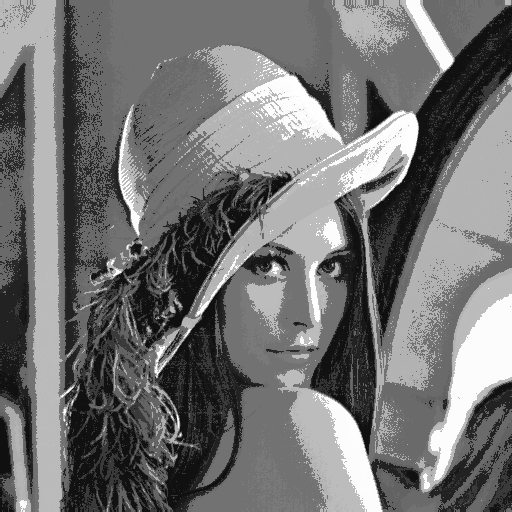
\includegraphics[width=\linewidth]{\detokenize{figuras/MSB.png}}
  \caption{MSB}
\end{subfigure}
 \end{center}
\end{figure}
\end{frame}
%-----------------------------------------------------------------------------
\subsection{Redes de Convolução}
\begin{frame}{Redes de Convolução}
\begin{figure}
    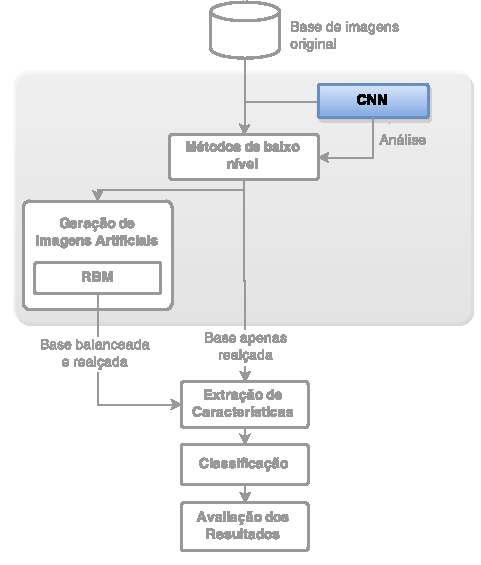
\includegraphics[height=0.75\textheight]{figuras/geral_cnn.pdf}
\end{figure}
\end{frame}
%-----------------------------------------------------------------------------
\begin{frame}{Redes Neurais}
\setstretch{1.2}
\setlength\leftmargini{0em}
\justifying
  \begin{itemize}
  \item Imagens como treinamento para inferir as regras para a classificação;
  \item Conhecimento através da experiência: ao tentar uma solução e errar, aprendem e podem tentar novamente;
  \item Aprendizado: ajuste dos pesos entre a saída esperada e a produzida.
  \end{itemize}
\end{frame}
%-----------------------------------------------------------------------------
\begin{frame}{Redes de Convolução - Deep Learning}
\setstretch{1.2}
\setlength\leftmargini{0em}
\justifying 
\begin{itemize}
  \item Reconhecimento humano de novos padrões - capacidade de generalização (hierarquias);% \cite{thesisDeep}. 
  \item Simular o funcionamento do cérebro humano por meio de camadas;
  \item Redes neurais profundas possuem duas ou mais ocultas; %\cite{neuralNielsen}. 
  \item Subdividem em problemas mais simples de serem resolvidos;
  \item Representam o estado da arte em visão computacional, mas está faltando o entendimento das suas propriedades.
%\cite{Schmidhuber2014}.
\end{itemize}
\end{frame}
%-----------------------------------------------------------------------------
\begin{frame}{Redes de Convolução}
\setstretch{1.2}
\setlength\leftmargini{0em}
\justifying
\textbf{Aprendem versões processadas das imagens de entrada: os filtros aprendidos são os que melhor diferenciam as classes.}
\vspace{1cm}
\begin{itemize}
  % \item Estado da arte da classificação, reconhecimento e localização de objetos;
  \item Multiplicações de um filtro espacial pela imagem de entrada, resultando em um \emph{mapa de características ativadas}; 
  \item Vetor de parâmetros capaz de aprender;
  % \item As características ativadas são diferentes;
  \item Um filtro é capaz de extrair apenas um tipo de característica;
  \item Camada de convolução = muitas convoluções em paralelo.
\end{itemize}
\end{frame}
%-----------------------------------------------------------------------------
\begin{frame}{Redes de Convolução}
 \begin{figure}[hbpt]
 \begin{center}
   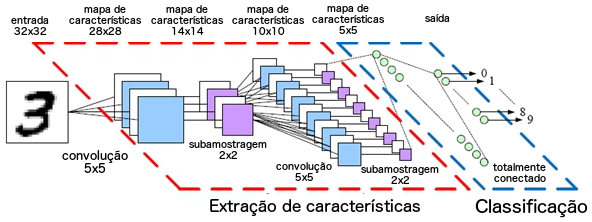
\includegraphics[width=0.9\linewidth]{figuras/CNNArchitecture.png}
 \end{center}
  \caption{Arquitetura de uma CNN. Fonte:~\tiny{\url{http://parse.ele.tue.nl/education/cluster2}}}
\end{figure}
\end{frame}
% A simulação desse modelo inspirado biologicamente utilizada hoje é de \citet{lecun1998} e chama-se Rede Neural de Convolução (CNN ou ConvNet). Eles simplificaram tal arquitetura para utilizar um algoritmo de retropropagação para o treino. Desde então, essas redes vêm sendo utilizadas para detecção, reconhecimento, restauração, remoção de ruído e segmentação de imagens e vídeos, além de sua aplicação em áudio. Um exemplo de utilização dessa rede inspirada no modelo de LeCun foi desenvolvida pela empresa Google, com o objetivo de detectar faces e placas de carros para proteger a privacidade nas imagens de StreetView \cite{google09}. 
\begin{frame}{Redes de Convolução}
 \begin{figure}[hbpt]
 \begin{center}
   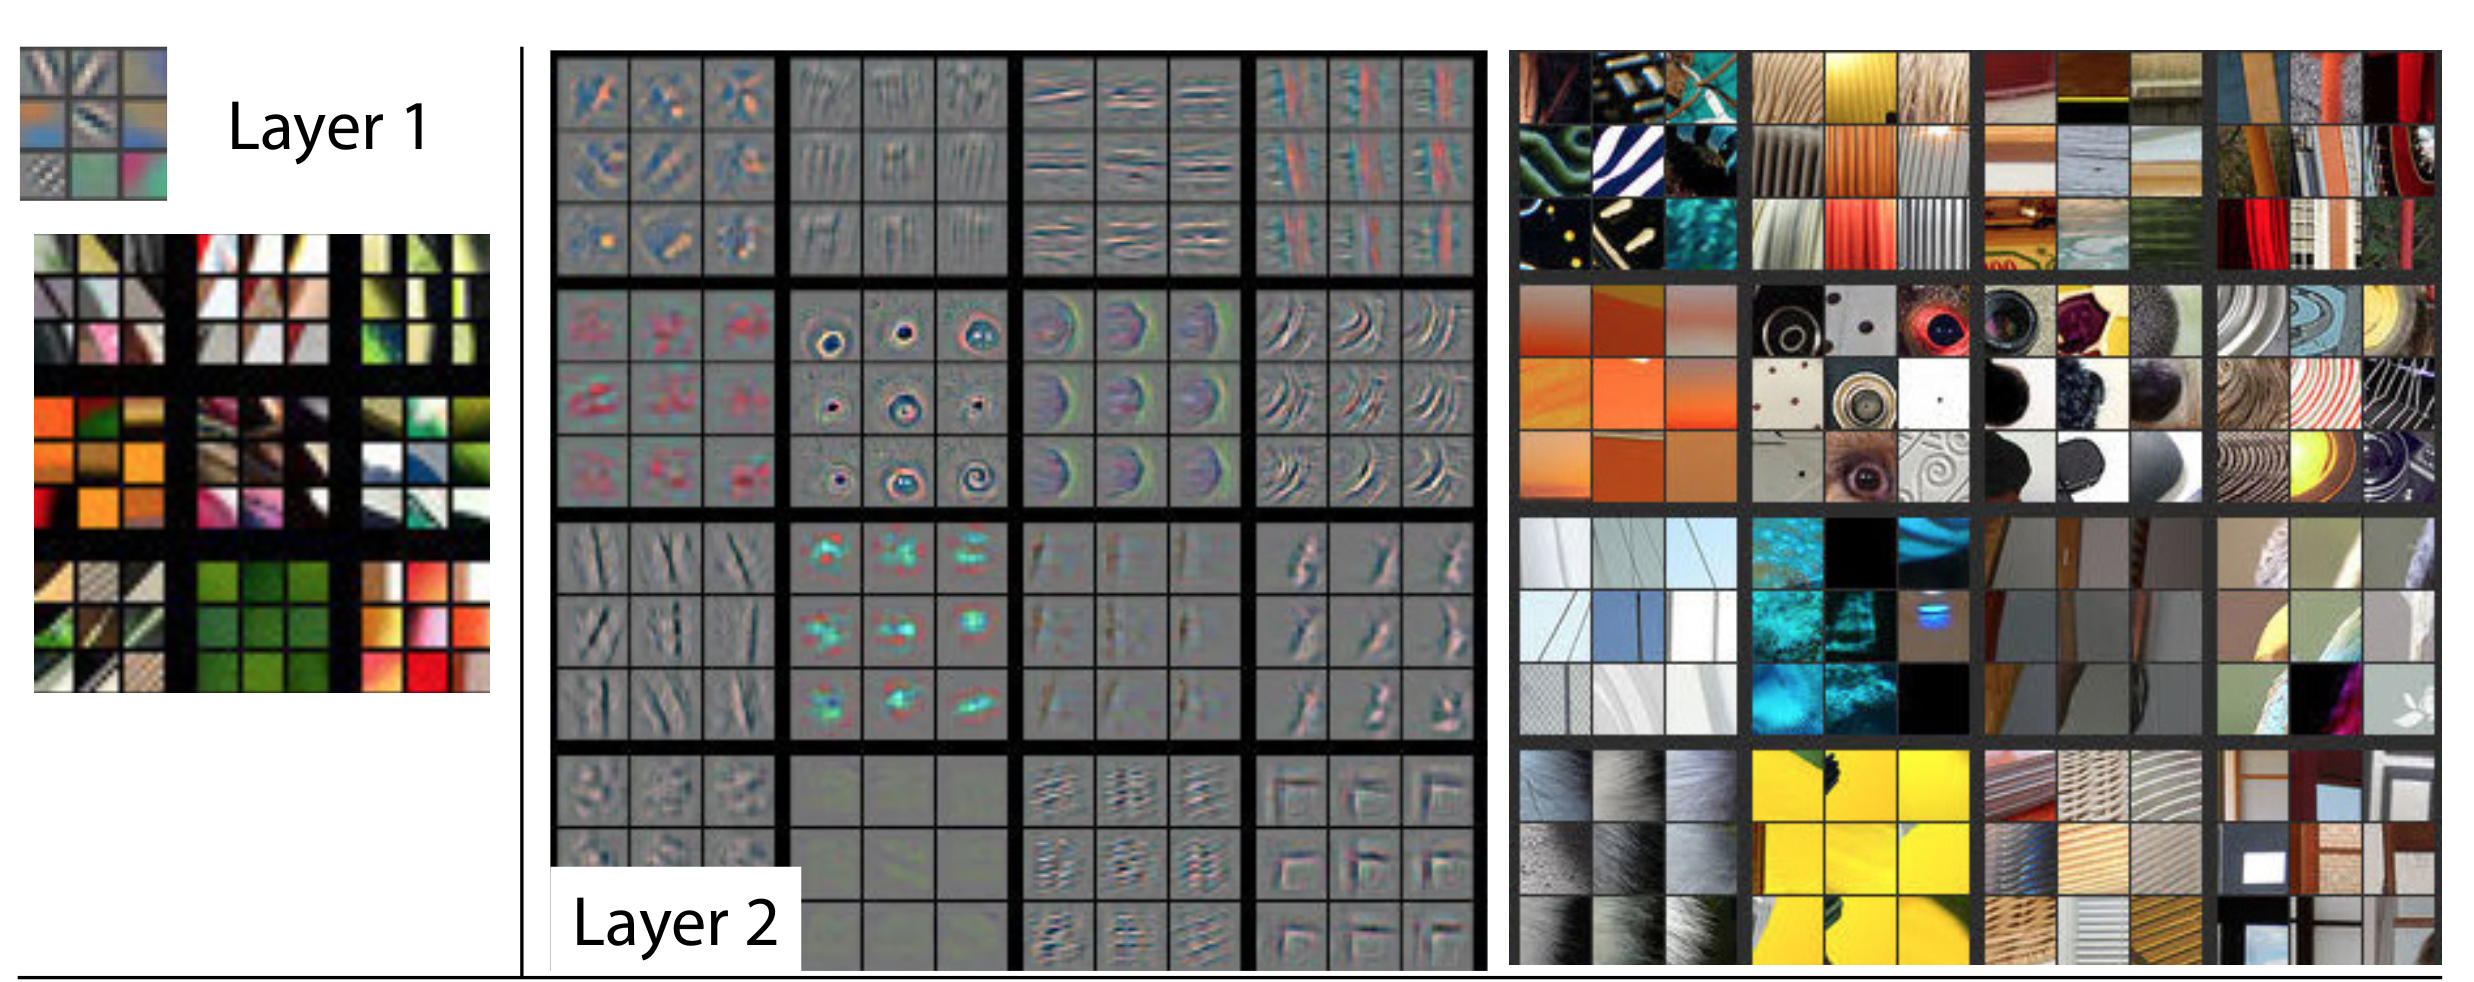
\includegraphics[width=0.9\linewidth]{{figuras/feature-1-2.png}}
  \caption{Primeira: ativar características de borda. Segunda camada: formas simples e texturas similares. Fonte:~\cite{Zeiler2013}}
 \end{center}
\end{figure}
\end{frame}
\begin{frame}{Redes de Convolução}
 \begin{figure}[hbpt]
 \begin{center}
   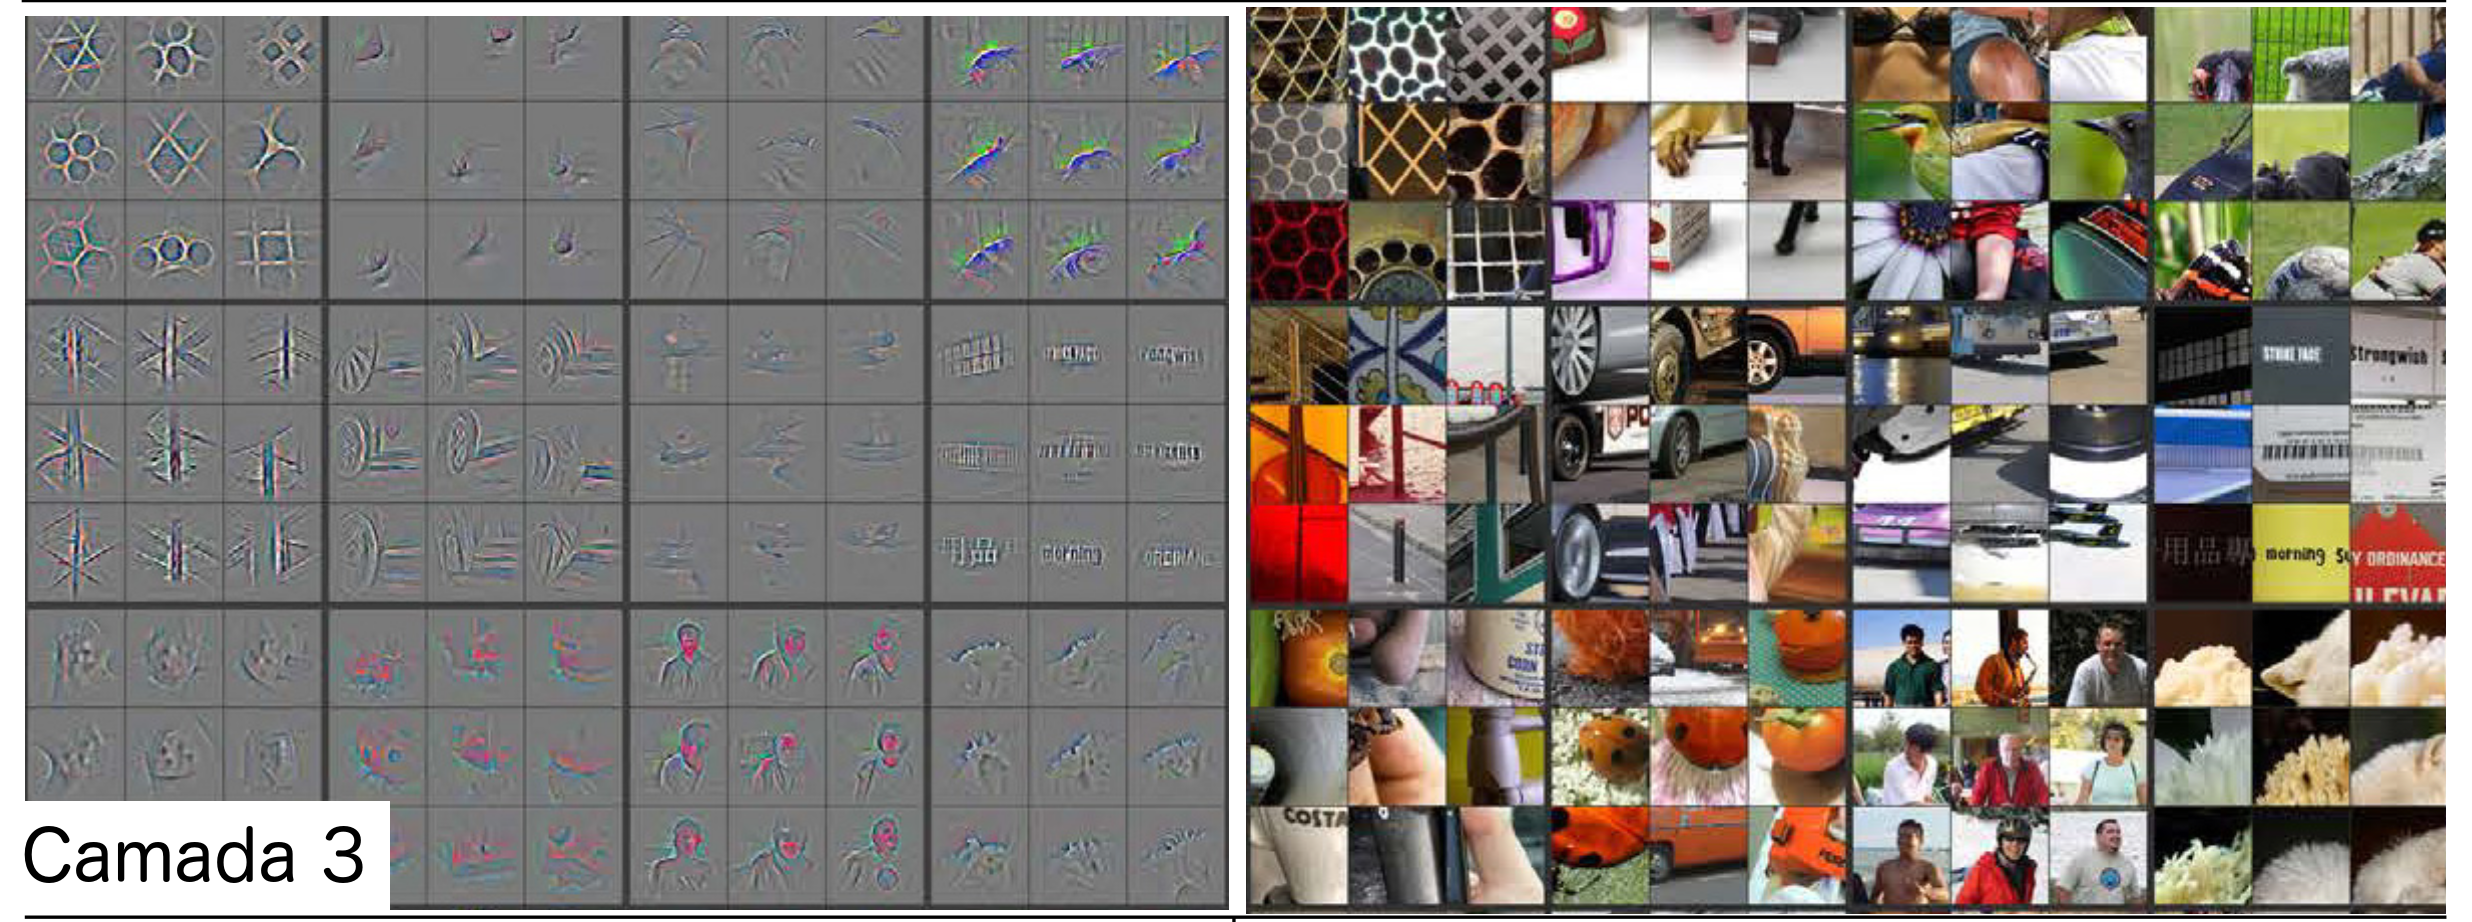
\includegraphics[width=0.9\linewidth]{{figuras/feature-3.png}}
  \caption{Terceira camada. Fonte:~\cite{Zeiler2013}}
 \end{center}
\end{figure}
\end{frame}
\begin{frame}{Redes de Convolução}
 \begin{figure}[hbpt]
 \begin{center}
   \includegraphics[width=0.9\linewidth]{{figuras/feature-4-5.png}}
  \caption{Quarta e quinta camada. Complexos pedaços das imagens ativados. Fonte:~\cite{Zeiler2013}}
 \end{center}
\end{figure}
\end{frame}
\begin{frame}{Redes de Convolução}
 \begin{figure}[hbpt]
 \begin{center}
   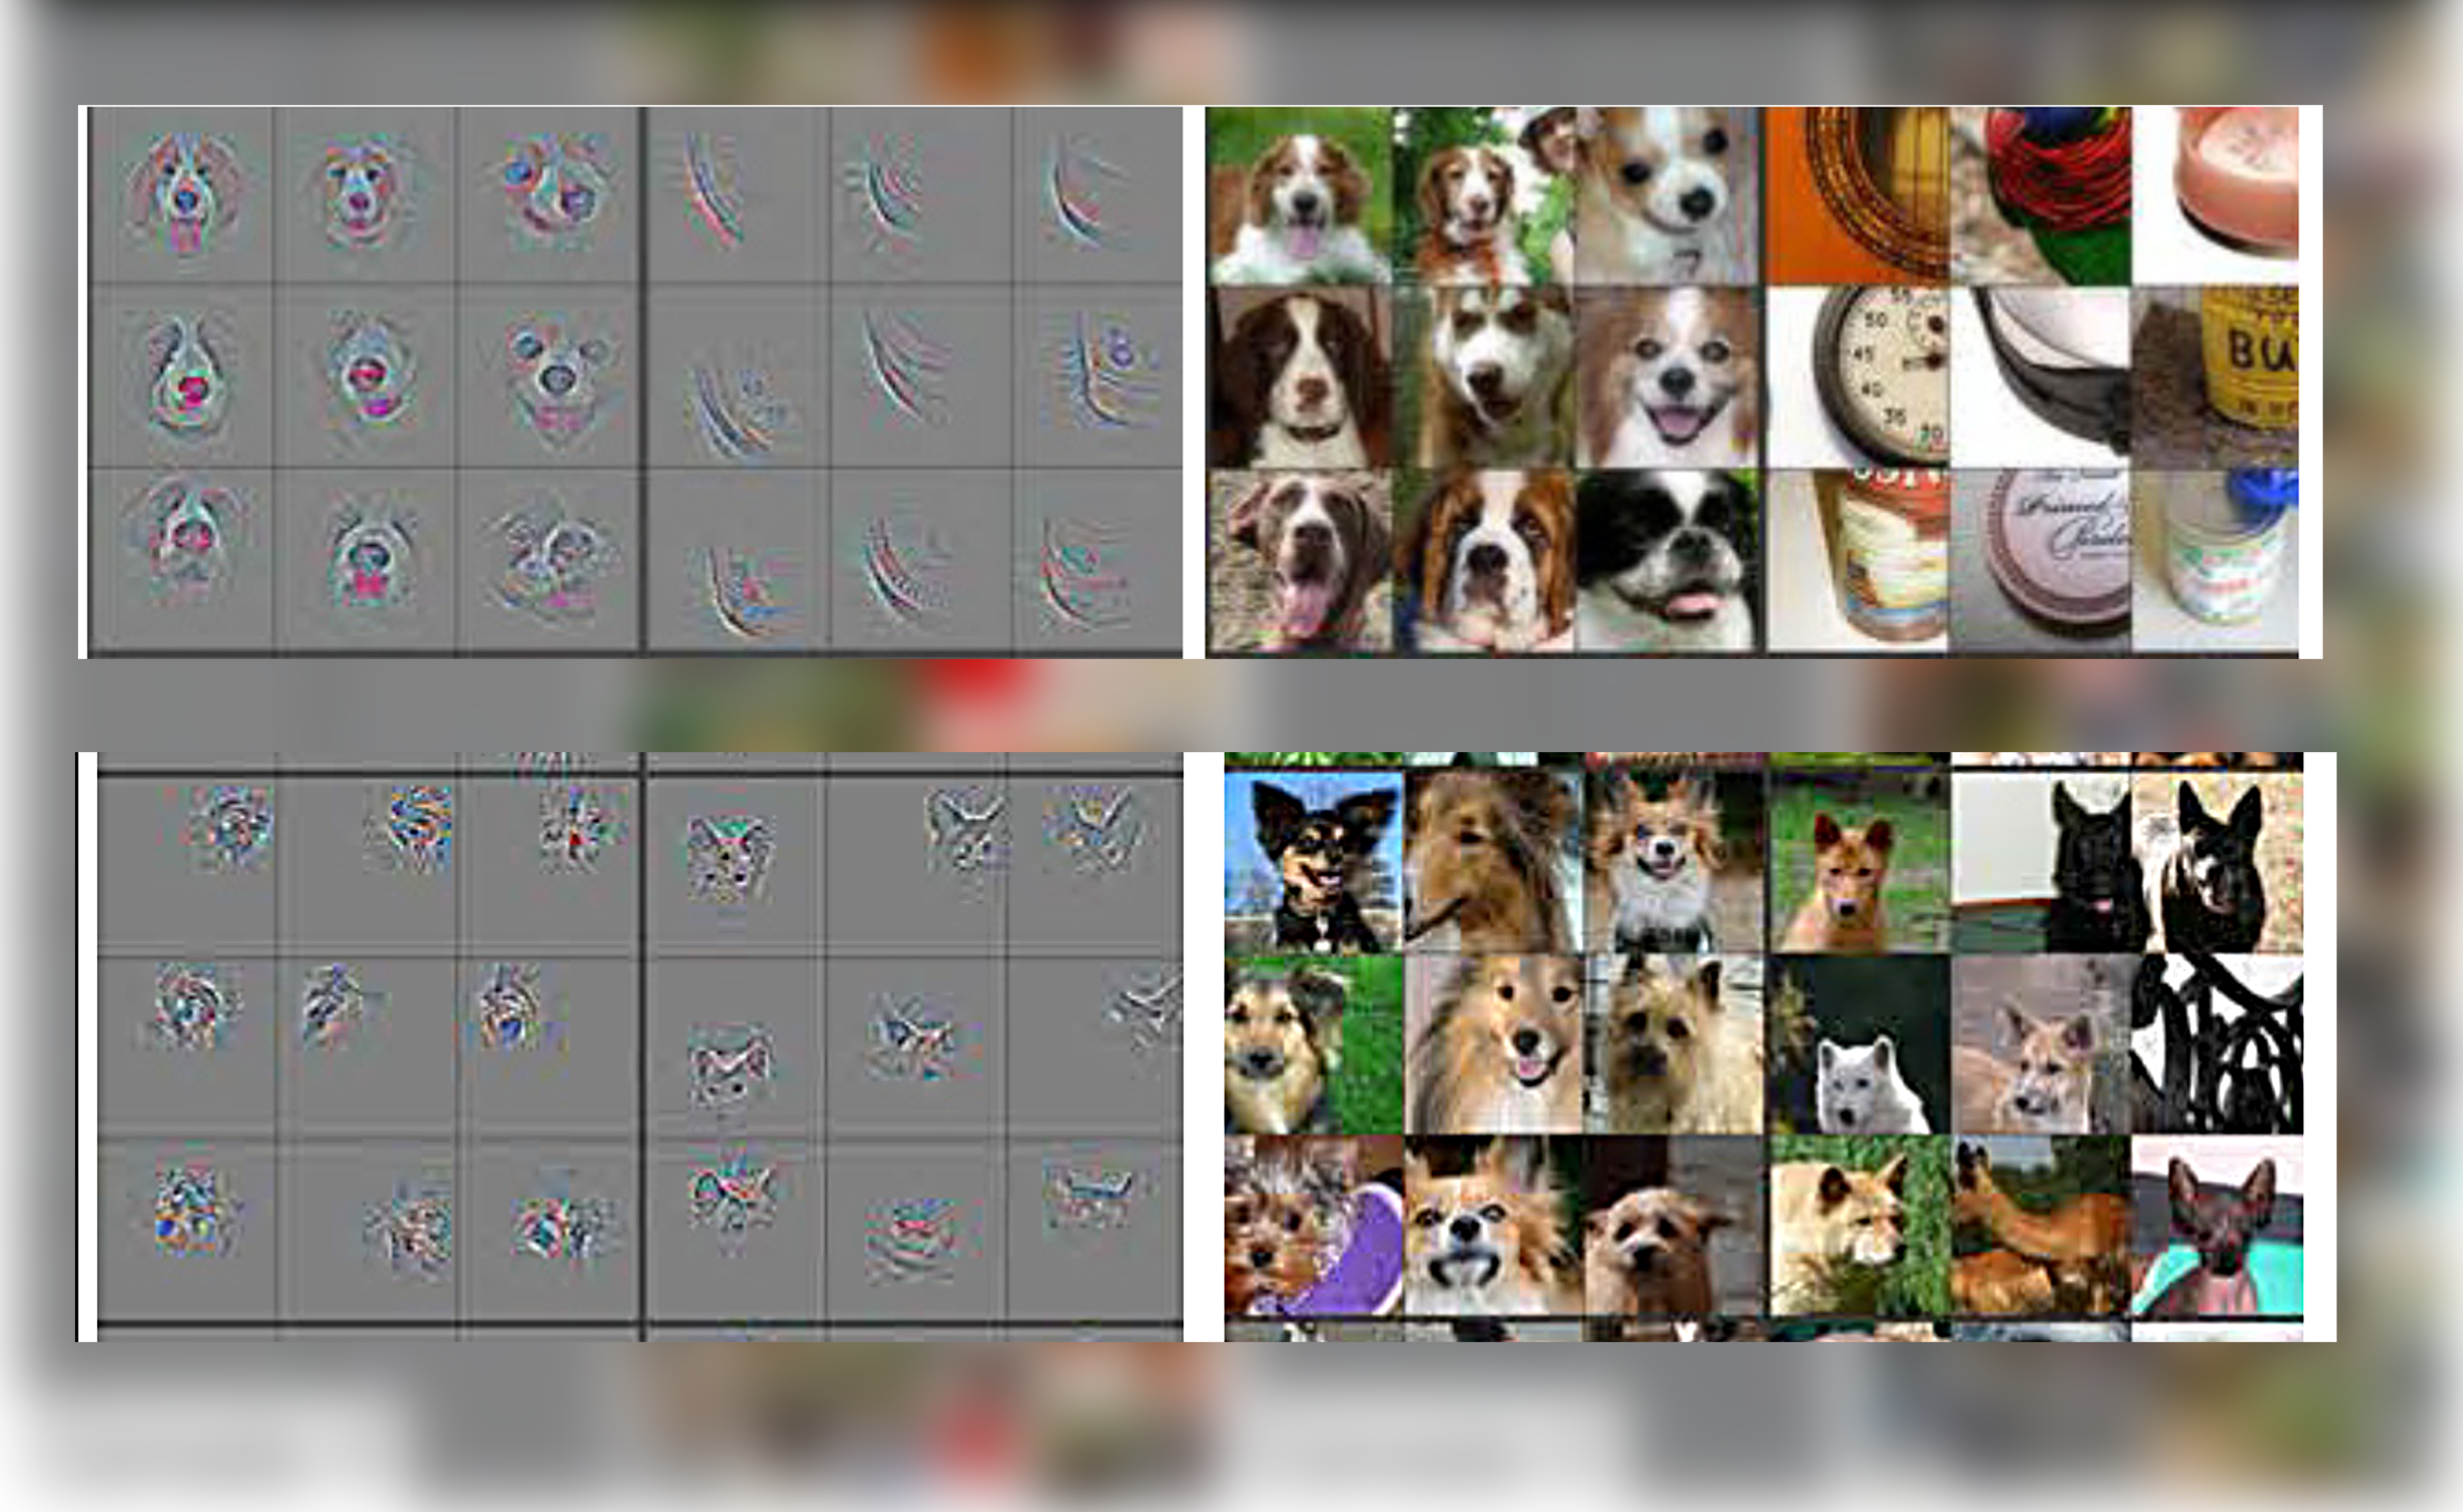
\includegraphics[width=0.9\linewidth]{{figuras/feature-4-5_blur.png}}
  \caption{Quarta e quinta camada. Insere abstração e invariância. Estruturas discriminantes. Fonte:~\cite{Zeiler2013}}
 \end{center}
\end{figure}
\end{frame}
%-----------------------------------------------------------------------------
\subsection{Desbalanceamento de classes}
\begin{frame}{Desbalanceamento de classes}
\begin{figure}
    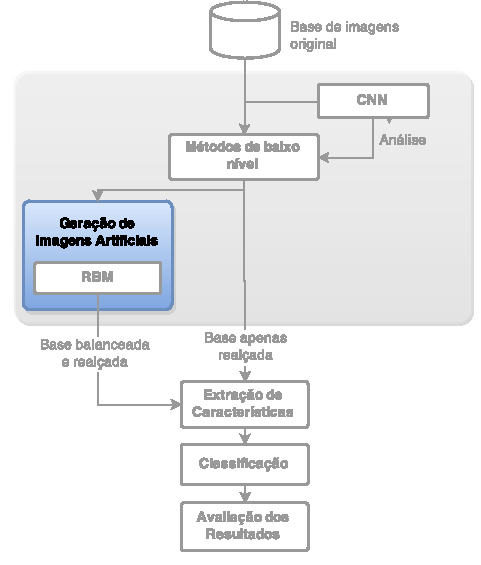
\includegraphics[height=0.75\textheight]{figuras/geral_geracao.pdf}
\end{figure}
\end{frame}
%-----------------------------------------------------------------------------
\begin{frame}{Desbalanceamento de classes}
\setstretch{1.2}
\setlength\leftmargini{0em}
\justifying
\setstretch{1.2}
\begin{itemize}
  \item Número desbalanceado de exemplos. Majoritárias x minoritárias.
  \item Abordagens:
    \begin{itemize}
        \item \emph{Modificar métodos de aprendizagem:} adicionar funções de custo na classificação;
        \item \emph{Pré-processamento ao reamostrar os dados:}
      \begin{itemize}
          \item Aumentar a minoritária;
          \item Diminuir a majoritária.
      \end{itemize}
    \end{itemize}
\end{itemize}
\end{frame}
%-----------------------------------------------------------------------------
\begin{frame}{Desbalanceamento de classes - Subamostragem}
\setlength\leftmargini{0em}
\justifying
    \begin{itemize}
        \item Diminuir o número de elementos do conjunto;
        \item Podem remover informações essenciais dos dados originais;
        \item Eliminar elementos distantes da fronteira de decisão;
        \item Normalmente apresentam resultados piores.
        % \item Não há melhor para todos os cenários.
    \end{itemize}
\end{frame}
%-----------------------------------------------------------------------------
\begin{frame}{Desbalanceamento de classes - Sobreamostragem}
\setlength\leftmargini{0em}
\justifying
    \begin{itemize}
        \item Aumentar o número de elementos;
        \item Replicar não reporta melhorias;
    \begin{block}{SMOTE}
\setlength\leftmargini{1em}
        \begin{itemize}
            \item Multiplica a diferença entre o vetor de características de um elemento e do seu vizinho mais próximo por um número [0-1];
            \item Adiciona ao vetor original, criando um novo elemento entre os dois vetores originais;
            \item Aprendido como exemplo da classe minoritária;
            \item Força uma região de decisão maior e mais geral;
        \end{itemize}
    \end{block}
    \end{itemize}
\end{frame}
%-----------------------------------------------------------------------------
\begin{frame}{Desbalanceamento de classes - SMOTE}
\setlength\leftmargini{0em}
\justifying
 \begin{figure}[hbpt]
 \begin{center}
   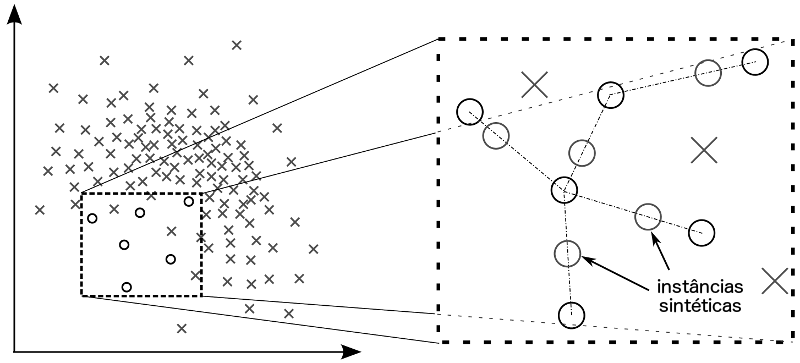
\includegraphics[width=.6\linewidth]{{figuras/smote.png}}
   % http://www.intechopen.com/books/advances-in-data-mining-knowledge-discovery-and-applications/selecting-representative-data-sets
 \end{center}
\end{figure}
\justifying
    \begin{itemize}
        \item Rebalancear ao gerar novos elementos, ao invés de replicá-los;
        \item Sobre os vetores de características previamente extraídos;
        \item (Chawla et al., 2002) \textbf{Diferentes estratégias para criar exemplos sintéticos podem melhorar a performance da classificação;}
        \item Utilizado para comparação.
    \end{itemize}
\end{frame}
%-----------------------------------------------------------------------------
\subsection{Máquina de Boltzmann restrita}
\begin{frame}{Máquina de Boltzmann restrita}
\begin{figure}
    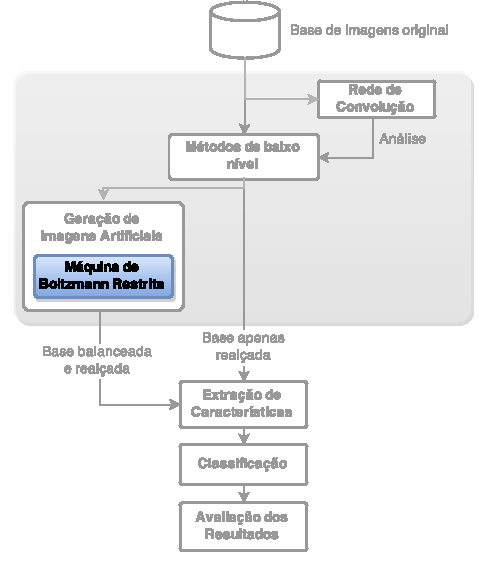
\includegraphics[height=0.75\textheight]{figuras/geral_rbm.pdf}
\end{figure}
\end{frame}
\begin{frame}{Máquina de Boltzmann restrita}
\setlength\leftmargini{0em}
\justifying
\begin{itemize}
  \item Pixels: unidades visíveis. Camada oculta: correlação entre os pixels;
  \item Aprendem representações das imagens;
  \item Verificação da relevância de uma imagem para o aprendizado;
  \item Utilizar apenas um neurônio oculto, com a matriz de pesos como memória associativa.
  \item Informação em uma imagem artificialmente gerada.
\end{itemize}
 \begin{figure}[hbpt]
 \begin{center}
   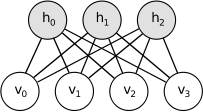
\includegraphics[width=.3\linewidth]{{figuras/rbm.png}}
 \end{center}
\end{figure}
\end{frame}
%-----------------------------------------------------------------------------
\begin{frame}{Redes Neurais}
\setstretch{1.2}
\setlength\leftmargini{0em}
\justifying
  \begin{itemize}
    \item Redes neurais de convolução (CNN)% - \cite{lecun1998})
    \begin{itemize}
    \item Compreendem todo o pipeline com camadas de neurônios;
    \item Aprendem as melhores características que diferenciam as classes, utilizando convolução;
    \end{itemize}
    \item Máquinas de Boltzmann restritas (RBM)
    \begin{itemize}
        \item Aprende a representação das imagens de entrada;
        \item Definir quais imagens são relevantes para o aprendizado.
    \end{itemize}
  \end{itemize}
\end{frame}
%-----------------------------------------------------------------------------
\subsection{Extração de características}
\begin{frame}{Extração de Características}
\begin{figure}
    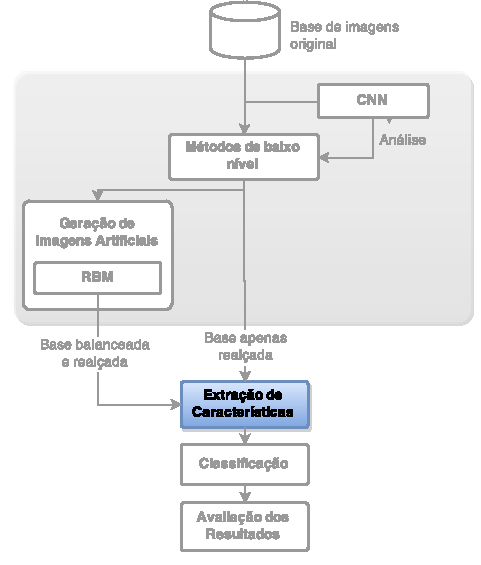
\includegraphics[height=0.75\textheight]{figuras/geral_extracao.pdf}
\end{figure}
\end{frame}
%-----------------------------------------------------------------------------
\begin{frame}{Extração de Características}
\setlength\leftmargini{0em}
\justifying
\begin{itemize}
\item Descrever as informações visuais relevantes em um vetor de características;
\item Entrada para o classificador de padrões;
% Exemplo: importante para a discriminação entre classes de algas é a forma. 
\item Salientar as diferenças entre imagens de classes distintas e suavizar possíveis diferenças de imagens da mesma classe (Ex. algas - forma).
\end{itemize}
\setlength\leftmargini{0em}
\begin{description}
\item [Textura:] suavidade, aspereza e uniformidade. Ex. entropia;
\item [Forma:] características externas. Ex. curvatura;
\item [Cor:] distribuição espacial de cores na imagem. Ex. histograma.
\end{description}
\end{frame}
%-----------------------------------------------------------------------------
\begin{frame}{Extração de Características}
\setlength\leftmargini{1.5em}
\begin{itemize}
\item[GCH]<1> {\emph{Histograma global de cor} - $N$ (intensidades).} % Mais simples representação. }

\item[CCV]<2> {\emph{Vetor de coerência de cor}. Classifica os pixels da imagem em coerentes e incoerentes de acordo com um \textit{threshold}, computa e concatena os histogramas - $2N$.}

\item[BIC]<3> {\emph{Classificação de pixels de borda e interior}. Mesma cor que seus vizinhos, é pixel de interior. Computa dois histogramas - $2N$.}

\item[ACC]<4> {\emph{Auto-correlograma de cor}: captura a correlação espacial entre cores idênticas. Probabilidade de encontrar dois pixels com a mesma cor, a uma distância $d$ um do outro. 1, 3, 5 e 7 - $4N$.}

\item[Haralick]<5> {Entropia, homogeneidade, contraste, correlação, probabilidade máxima e uniformidade - $6$.}
\end{itemize}
\end{frame}
%-----------------------------------------------------------------------------
\section{Metodologia}
\begin{frame}{Metodologia - Pesquisa Bibliográfica}
\setstretch{1.2}
\setlength\leftmargini{0em}
\justifying
\begin{itemize}
\item Características latentes; 
\item Redes neurais CNN e RBM;
\item Desbalanceamento de classes;
\item Descritores de características;
\item Classificador de padrões.
\end{itemize}
\end{frame}
%-----------------------------------------------------------------------------
\begin{frame}{Metodologia - Implementação}
\setstretch{1.2}
\setlength\leftmargini{1em}
\begin{block}{}
\justifying
\begin{itemize}
\item Biblioteca OpenCV; %\cite{Intel2010}. 
\item Linguagens de programação C++ e Python;
\item Código disponível em \footnotesize{\url{https://bitbucket.org/moacirponti/imagefeatureextraction/overview}}. 
\end{itemize}
\end{block}
\end{frame}
%-----------------------------------------------------------------------------
\begin{frame}{Metodologia - Bases de Imagens}
\setstretch{1.2}
\setlength\leftmargini{1em}
\begin{block}{}
\justifying
\begin{itemize}
\item Viés genérico: diversas coleções de imagens com o objetivo de estabelecer ou refutar as hipóteses levantadas;
\item Resultados preliminares com a base de imagens COREL\footnote{Disponível em http://wang.ist.psu.edu/docs/related/};
\end{itemize}
\end{block} 
 \begin{figure}[hbpt]
 \begin{center}
   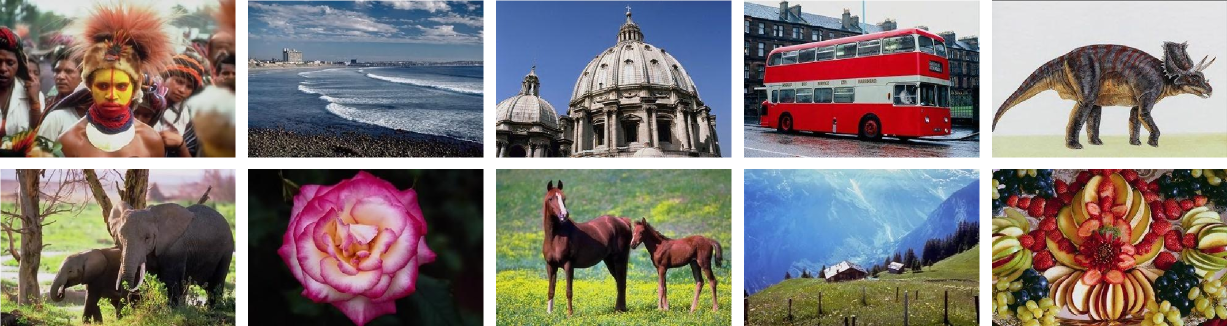
\includegraphics[width=0.8\linewidth]{\detokenize {figuras/exemplos_corel.png}}
 \end{center}
  \caption{Base de imagens COREL-1000}
\end{figure}
\end{frame}
%-----------------------------------------------------------------------------
\begin{frame}{Metodologia - Bases de Imagens}
\setstretch{1.2}
\setlength\leftmargini{1em}
\begin{block}{Bem discriminadas}
\justifying
\begin{itemize}
\item Cor: COREL-1000;
\item Textura: Describable Textures Dataset\footnote{http://www.robots.ox.ac.uk/~vgg/data/dtd/} (DTD);
\item Forma: Leafsnap\footnote{http://leafsnap.com/dataset/};
\end{itemize}
\end{block}
\vspace{1em}
\begin{columns}
  \begin{column}{0.5\textwidth}
    \begin{figure}[hbpt]
      \begin{center}
        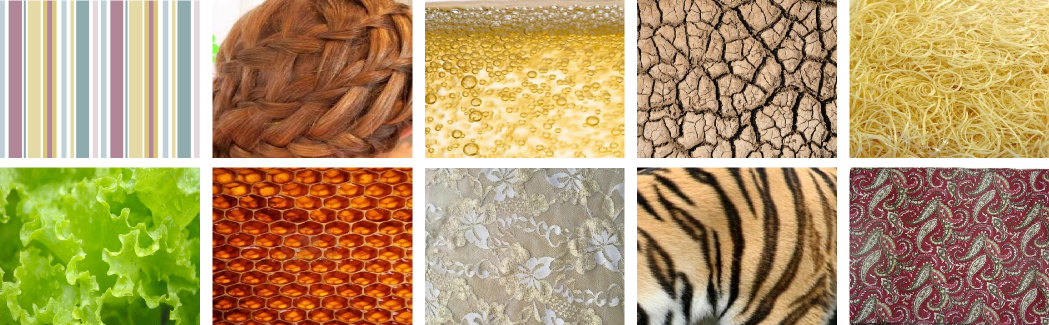
\includegraphics[width=\columnwidth]{figuras/texture.png}
      \end{center}
      \caption{DTD.}
    \end{figure}
    \end{column}
  \begin{column}{0.5\textwidth}
    \begin{figure}[hbpt]
      \begin{center}    
        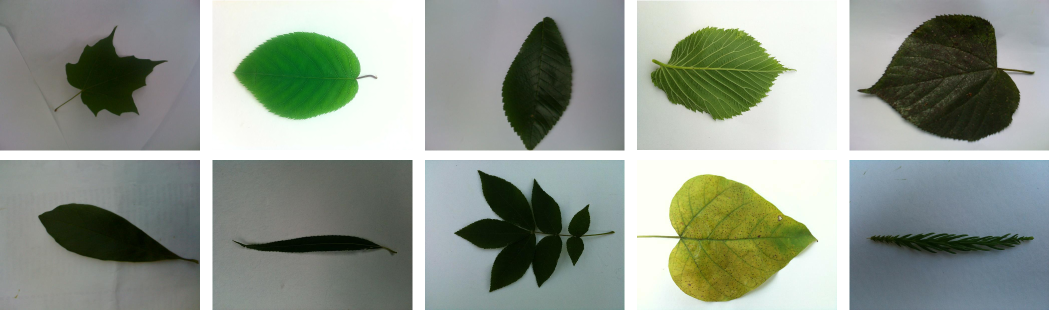
\includegraphics[width=\columnwidth]{figuras/leafs.png}
       \end{center}
      \caption{Leafsnap.}
    \end{figure}
  \end{column}
\end{columns}
\end{frame}
%-----------------------------------------------------------------------------
\begin{frame}{Metodologia - Experimentos}
\setstretch{1.2}
\setlength\leftmargini{1em}
\begin{block}{}
\justifying
\begin{itemize}
\item Explorar algoritmos de realce de características relevantes:
\begin{itemize}
\item Melhorar discriminação entre as classes;
\item Auxiliar no rebalanceamento.
\end{itemize}
\item Entrada: imagens originais das coleções disponíveis na literatura;
\item Resultado: medidas estatísticas da classificação.
\end{itemize}
\end{block}
\end{frame}
%----------------------------------------------------------------------------- 
\begin{frame}{Metodologia - Análise dos resultados}
\setstretch{1.2}
\setlength\leftmargini{1em}
\begin{block}{}
\justifying
\begin{itemize}
\item Comparar a classificação:
\begin{itemize}
\item Base original;
\item Base realçada pelo método proposto.
\end{itemize}
\item Comparar os métodos:
\begin{itemize}
\item Geração artificial;
\item Técnicas de sobreamostragem disponíveis na literatura, como o SMOTE.
\end{itemize}
\end{itemize}
\end{block}
\end{frame}
% a medida estatística mais comum para avaliação é a razão do número de acertos pela quantidade de imagens testadas. Essa medida, conhecida por \underline{acurácia}, pode não refletir propriamente os resultados, em um cenário de bases desbalanceadas. Isso se deve ao fato de que se a classe minoritária não obtiver nenhum resultado correto e a classe majoritária tiver 100\% de acertos, a acurária normal poderá ser muito alta, mesmo considerando que nenhuma imagem da classe minoritária foi corretamente classificada. Dessa forma, considera que os erros são igualmente importantes. Mas em se tratando de bases desbalanceadas, deve-se diferenciar o erro em, por exemplo, diagnosticar um paciente doente -- classe minoritária -- como sendo saudável e um paciente saudável -- classe majoritária -- como estando doente \cite{Batista2004}. No primeiro caso, o paciente corre risco de diagnóstico tardil, enquanto o paciente saudável realiza outros testes para refutação.

% Pode-se estender essa medida obtendo-se a \underline{acurácia $k$-fold}: medida de acerto baseada na divisão do conjunto de objetos em teste e treinamento, realizando a repetição dos experimentos $n$ vezes e obtendo a média e o desvio padrão. A acurácia de cada experimento é obtida pela Equação~\ref{eq:Accuracy}, que considera problemas de desbalanceamento de classes.
%-----------------------------------------------------------------------------
\begin{frame}{Metodologia - Avaliação}
% \setstretch{1.2}
\setlength\leftmargini{1em}
\begin{block}{Medida F1}
\justifying
Problema da acurácia: minoritária sem resultados corretos. \\
% Performance da classificação em cenários desbalanceados.
\begin{itemize}

\item Precisão (exatidão): dos exemplos classificados como positivos, quantos realmente são.
\vspace{-1.5em}
\begin{equation*}
  P = \frac{VP}{VP + FP}
\end{equation*}
\item Revocação (completude): exemplos positivos corretamente classificados como tal. 
\begin{equation*}
  R = \frac{VP}{VP + FN}
\end{equation*}

\pause
\begin{equation*}
  F1 = 2 \frac{PR}{P+R}
\end{equation*}
\end{itemize}
\end{block}
\end{frame}
%-----------------------------------------------------------------------------
% Uma outra medida para bases desbalanceadas é a \underline{medida-F1} (conhecida como \textit{F1-Measure} ou \textit{F1-Score} e apresentada na Equação~\eqref{medidaf}), que combina precisão e revocação como medida de 
% A partir dessas medidas, o \underline{teste estatístico de Friedman} pode ser usado para determinar se há diferença significante em uma amostra de resultados gerados \cite{friedman2010}. As performances dos algoritmos são analisados e um \textit{rank} é atribuído para cada conjunto de dados. Ele considera que a hipótese nula a ser testada é que não há diferença estatística relevante entre as observações. Para analisar se o teste da hipótese é significativo, pode ser utilizado o \underline{p-valor}, que indica o quão estatisticamente significante o resultado é: quanto menor o seu valor, maior a evidência contra a hipótese nula (geralmente o limiar utilizado é de 0,05).

\begin{frame}{Metodologia - Avaliação}
\setstretch{1.2}
\setlength\leftmargini{1em}
\begin{block}{Teste de Friedman}
\begin{itemize}
\item Determinar se há diferença significante entre os resultados gerados;
\item Analisa as performances dos algoritmos e atribui um \textit{rank};
\item A hipótese nula a ser testada é que não há diferença estatística relevante entre as observações;
\item P-valor indica essa significância: quanto menor o seu valor, maior a evidência contra a hipótese nula (limiar de 0,05).
\end{itemize}
\end{block}
\end{frame}
%-----------------------------------------------------------------------------
\begin{frame}{Metodologia - Avaliação}
\setstretch{1.2}
\justifying
\setlength\leftmargini{1em}
\begin{block}{Mahalanobis}  %\cite{mahalanobis2000}
Distância entre a média e a variância das classes. 
\vspace{4pt}

Baseia na correlação entre as variáveis e pode ser definida por
\begin{equation*}
  D_m(x_i) = \sqrt{(x_i - \mu)C^{-1}(x_i-\mu)^T},
\end{equation*}
\noindent onde $x_i$ é um vetor de valores, $\mu$ a média e C a matriz de covariância.
\end{block}
\end{frame}
%%%%%%%%%%%%%%%%%%%%%%%%%%%%%%%%%%%%%%%%%%%%%%%%%%%%%%%%%%%%%%%%%%%%%%%%%%%%%%%
\section{Resultados}
\subsection{Resultados Esperados}
\begin{frame}{Resultados Esperados}
\setlength\leftmargini{0em}

\begin{itemize}
\item Melhorar a classificação, validando-a com a medida-F1. 
\begin{itemize}
\item \textit{Pré-processamento} de imagens que caracterizem melhor aspectos de suas classes;
\item \textit{Geração artificial de imagens} de classes minoritárias.
\end{itemize}
\item Analisar as características aprendidas com a CNN em bases específicas; 
\item Escolher imagens que adicionam informações (RBM);
\item Testar bases naturalmente não balanceadas.
\end{itemize}

% Os resultados esperados são relacionados às áreas de \textbf{processamento de imagens e reconhecimento de padrões}. Espera-se obter uma comprovação das hipóteses levantadas por essa pesquisa. Os resultados são esperados em duas vertentes:

% \begin{enumerate}
%  \item \textit{Pré-processamento} de imagens que caracterizem melhor aspectos de suas classes, aumentando a variância entre as classes quando comparado com as imagens originais.
%  \item \textit{Geração artificial de imagens} de classes minoritárias de forma a compensar o desbalanceamento natural das bases de dados.
% \end{enumerate}

% Em ambos os casos pretende-se melhorar a classificação, validando-a através do cálculo da medida-F1. A análise das características aprendidas por uma rede neural de convolução será realizada ao executar o treinamento com bases específicas que destaquem propriedades como cor, textura e forma. Além disso, os resultados serão obtidos a partir da escolha de quais imagens adicionam informação ao conjunto de treino. As redes RBM serão utilizadas para este fim. Bases naturalmente não balanceadas serão testadas e seus resultados avaliados.
\end{frame}
%-----------------------------------------------------------------------------
\subsection{Descrição do experimento}
\begin{frame}{Descrição do Experimento}
\setlength\leftmargini{1em}
\setstretch{1.2}
\renewcommand{\tabcolsep}{0.04cm}
\begin{figure}[!h]
 \begin{center}
 \begin{tabular}{ccccc}
   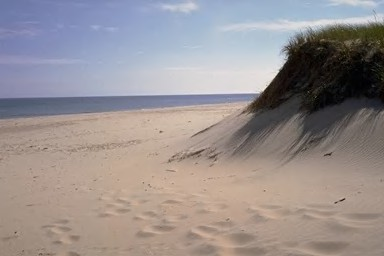
\includegraphics[width=0.245\linewidth]{\detokenize {figuras/original-1.jpg}}&
   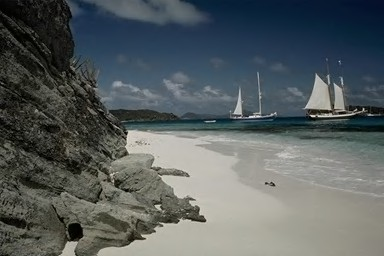
\includegraphics[width=0.245\linewidth]{\detokenize {figuras/original-2.jpg}}&
   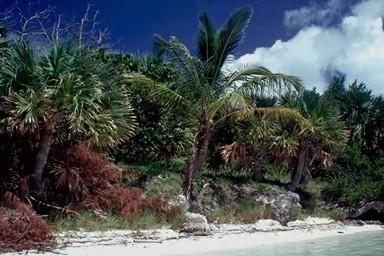
\includegraphics[width=0.245\linewidth]{\detokenize {figuras/original-3.jpg}}&
   % 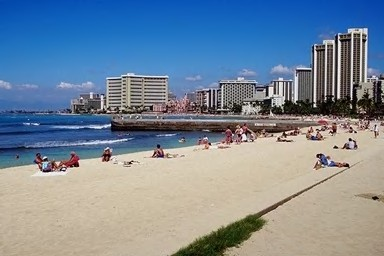
\includegraphics[width=0.19\linewidth]{\detokenize {figuras/original-4.jpg}}&
   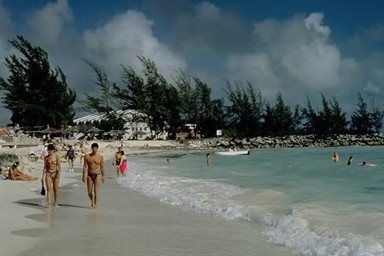
\includegraphics[width=0.245\linewidth]{\detokenize {figuras/original-5.jpg}}\\
   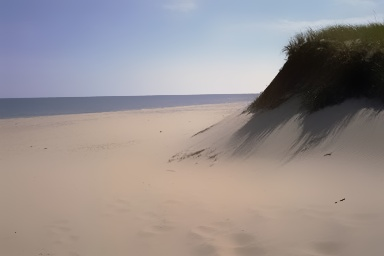
\includegraphics[width=0.245\linewidth]{\detokenize {figuras/gerada-1_blur.jpg}}&
   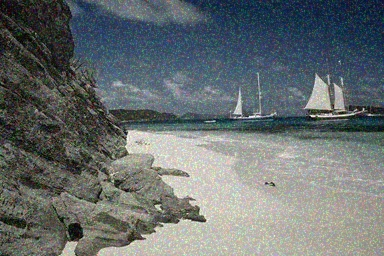
\includegraphics[width=0.245\linewidth]{\detokenize {figuras/gerada-2_ruido.jpg}}&
   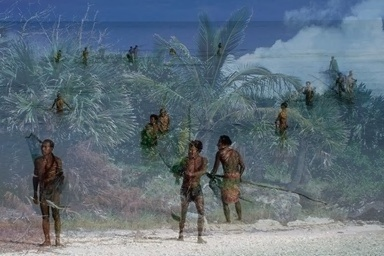
\includegraphics[width=0.245\linewidth]{\detokenize {figuras/gerada-3_blend.jpg}}&
   % 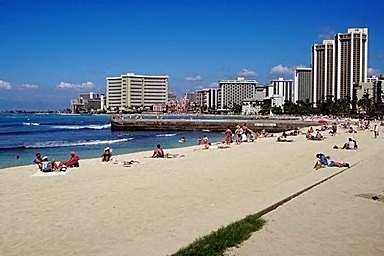
\includegraphics[width=0.19\linewidth]{\detokenize {figuras/gerada-4_unsharpMask.jpg}}&
   \includegraphics[width=0.245\linewidth]{\detokenize {figuras/gerada-5.jpg}} \\
 \end{tabular}
 \end{center}
  \caption{Geração de imagens artificiais para o rebalanceamento de classes por meio de: borramento, adição de ruído, mistura e combinação.}
\end{figure}
\renewcommand{\tabcolsep}{0.5cm}
\vspace{25pt}
\end{frame}
%-----------------------------------------------------------------------------
% Os descritores de características utilizados para os resultados foram apresentados na Seção \ref{sec:extracao}. Considerando que em um experimento anterior o melhor resultado foi atribuído à quantização com o método de Intensidade para o extrator Haralick e MSB para os outros, apenas esses testes foram aprofundados (tópico anteriormente discutido na Seção \ref{sec:quantizacao}). Neste experimento o classificador KNN foi utilizado, com $K=1$. Inicialmente o classificador Naive Bayes foi explorado, apresentando melhora na acurácia ao apenas replicar as imagens. Esse comportamento não é desejado em um classificador para a avaliação de rebalanceamento de classes. O código desenvolvido para esses resultados preliminares está disponível em \url{https://bitbucket.org/moacirponti/imagefeatureextraction/overview}. 
\begin{frame}[plain]{Descrição do Experimento}
\begin{figure}[!htb]
 \begin{center}
   \includegraphics[width=0.65\textheight]{\detokenize {figuras/flow_main.pdf}}
 \end{center}
  \caption{Fluxo dos resultados preliminares.}
\end{figure}
\end{frame}
%-----------------------------------------------------------------------------
\begin{frame}[plain]{Descrição do Experimento}
\begin{figure}[!htb]
 \begin{center}
   \includegraphics[width=0.55\textheight]{\detokenize {figuras/flow_sub.pdf}}
 \end{center}
  \caption{Fluxo da geração artificial.}
\end{figure}
\end{frame}
%-----------------------------------------------------------------------------
\subsection{Resultados Preliminares}
\begin{frame}{Resultados Preliminares}
\setlength\leftmargini{0em}
\setstretch{1.2}
\justifying
Classes com maior dificuldade de diferenciação, havendo alta taxa de sobreposição de intensidades de cores e texturas.
\begin{figure}[!htb]
 \begin{center}
   \includegraphics[width=\linewidth]{\detokenize {figuras/praia-montanha.png}}
 \end{center}
  \caption{Classes ``praia'' e ``montanha'' da base de imagens COREL-1000.}
\end{figure}
\end{frame}
%-----------------------------------------------------------------------------
\begin{frame}{Resultados Preliminares - Melhor}
\setlength\leftmargini{0em}
\justifying
\begin{itemize}
\item Ganho estatístico da medida-F, quando comparado à geração de exemplos artificiais no espaço de atributos; % (ou seja, depois que as características já foram extraídas das imagens)
% \item Descritor ACC, conversão MSB e operação de pré-processamento combinação. 
\end{itemize}
\vspace{-0.3cm}
\begin{figure}[htb]
 \begin{center}
   \includegraphics[width=0.7\linewidth]{\detokenize {figuras/resultado-melhor4.png}}
 \end{center}
 \caption{Resultado obtido com a operação de combinação.}
\end{figure}
\end{frame}
%-----------------------------------------------------------------------------
\begin{frame}{Resultados Preliminares - Pior}
\setlength\leftmargini{0em}
\setstretch{1.2}
\justifying
\begin{figure}[htb]
 \begin{center}
   \includegraphics[width=0.8\linewidth]{\detokenize {figuras/resultado-pior1.png}}
 \end{center}
 \caption{Piores resultados, obtidos com a adição de ruído.}
\end{figure}
% \begin{itemize}
% % \item Adição de ruído, extração com CCV e a quantização por MSB;
% \end{itemize}
\end{frame}
%-----------------------------------------------------------------------------
\begin{frame}{Resultados Preliminares}
\setlength\leftmargini{0em}
\setstretch{1.2}
\justifying
\begin{itemize}
\item Melhores operações: todas, apenas mistura e apenas composição;
\item Piores: apenas borramento, ruído e \textit{unsharp masking} (filtros comuns);
\vspace{2pt}
\item Melhor descritor: ACC;
\item Piores: CCV e GCH;
% \vspace{2pt}
% \item Melhor quantizador: MSB;
% \item Piores: CCV e GCH;
\end{itemize}
\end{frame}
%-----------------------------------------------------------------------------
\begin{frame}{Resultados Preliminares}
\setlength\leftmargini{0em}
\setstretch{1.2}
\justifying
\begin{itemize}
\item Teste de Friedman para todas as execuções das melhores operações;
\item P-valor = $4.24E^{-11}$; Hipótese nula rejeitada.
\end{itemize}
\begin{table}[htb]
\centering
\caption{Posição média dos algoritmos utilizando Friedman}
  \begin{tabular}{c|c}
    Algoritmos  &   Posição \\ \hline
    Artificial  &   1.3863  \\
    Smote       &   1.6136  \\
    Original    &   3.0000  \\
  \end{tabular}
\end{table}
\begin{itemize}
\item Em algumas execuções: Artificial (1), SMOTE (2) e Original (3).
\end{itemize}
\end{frame}
%-----------------------------------------------------------------------------
\begin{frame}{Resultados Preliminares}
\setlength\leftmargini{0em}
% \setstretch{1.2}
\justifying

\begin{itemize}
\item Replicação: SRS - \textit{Simple Random Sampling};
\item Não adiciona informações novas para o aprendizado.
\end{itemize}

\begin{figure}[htb]
 \begin{center}
   \includegraphics[width=0.65\linewidth]{\detokenize {figuras/resultado-copia.png}}
 \end{center}
  \caption{Simples replicação de exemplos sem pré-processamento.}
\end{figure}
\end{frame}
%%%%%%%%%%%%%%%%%%%%%%%%%%%%%%%%%%%%%%%%%%%%%%%%%%%%%%%%%%%%%%%%%%%%%%%%%%%%%%%
\begin{frame}{Resultados Preliminares - Rede de Convolução}
\begin{table}
\url{http://caffe.berkeleyvision.org/}
\caption{Treinamento das classes praia e montanha da base COREL-1000.}
  \begin{tabular}{c|c}
    Bases    &   Medida F1 \\ \hline
    Original      &   0.708  \\
    Desbalanceada &   0.577  \\
    Rebalanceada  &   0.677  \\
  \end{tabular}
\end{table}
\end{frame}
%%%%%%%%%%%%%%%%%%%%%%%%%%%%%%%%%%%%%%%%%%%%%%%%%%%%%%%%%%%%%%%%%%%%%%%%%%%%%%%
% O treinamento de uma rede neural de convolução~\footnote{\url{http://caffe.berkeleyvision.org/}} foi realizado, utilizando as classes ``praia'' e ``montanha'', balanceadas, da base COREL-1000. A classificação desse treinamento obteve $\approx 80\%$ de acurácia, enquanto que utilizando os extratores padrões foi possível atingir apenas $\approx 69\%$. Isso reforça a proposta de analisar quais são as características latentes que esse tipo de rede neural consegue extrair. Para essa análise vão ser utilizadas bases discriminadas quanto às propriedades de textura, cor e forma.

% Além de analisar o processamento realizado por uma rede de convolução para a classificação das imagens, uma rede RBM também será treinada para análise da sua memória associativa. As imagens artificialmente geradas foram adicionadas no conjunto de treino sem verificação da sua relevância, o que pode ter prejudicado a classificação. A memória associativa aprendida com o treinamento de uma máquina de Bolztmann restrita pode vir a auxiliar no entendimento dessas imagens como relevantes ou não. Além disso, pode servir como escolha para qual imagem original utilizar, ao invés do método aleatório utilizado nos resultados preliminares.

\section{Próximos Passos}
\begin{frame}{Próximos Passos - Curto Prazo}
\setlength\leftmargini{0em}
\setstretch{1.2}
\justifying
  \begin{itemize}
  \item Desbalancear as 10 classes da COREL-1000 em escada;
  \item Utilizar todas as classes com apenas 1 desbalanceada;
  \item Analisar as características latentes que as redes neurais de convolução conseguem extrair.
    \begin{itemize}
      \item Bases bem discriminadas quanto às propriedades de textura, cor e forma.
    \end{itemize}
  \end{itemize}
\end{frame}
%-----------------------------------------------------------------------------
\begin{frame}{Próximos Passos - Médio Prazo}
\setlength\leftmargini{0em}
\setstretch{1.2}
\justifying
  \begin{itemize}
  \item Analisar a memória associativa de uma máquina de Boltzmann restrita.
  \begin{itemize}
    \item Escolher para qual imagem original utilizar, ao invés do método aleatório utilizado nos resultados preliminares;
    \item Verificação da relevância das imagens geradas.
  \end{itemize}
  \end{itemize}
\end{frame}
%-----------------------------------------------------------------------------
\section{Atividades e cronograma}
\begin{frame}{Atividades e Cronograma}
\definecolor{cinza}{rgb}{0.5,0.5,0.5}
\newcommand{\y}{\color{black}\rule{20pt}{7pt}}
\newcommand{\x}{\hspace*{20pt}}
\renewcommand{\r}{\color{cinza}\rule{20pt}{7pt}}
% \setlength{\tabcolsep}{0pt}
\begin{table}
\caption{Duração de cada atividade a partir de 24/02/2014.}
\begin{center}
\resizebox{\columnwidth}{!}{%
\begin{tabular}{|c|c|c|c|c|c|}
 \cline{2-6}
\multicolumn{1}{l|}{} & \multicolumn{2}{c|}{2014} & \multicolumn{2}{c|}{2015} & 2016 \\
\hline \ Atividade\ \ & 1\textordmasculine\ Sem. & 2\textordmasculine\
Sem. & 1\textordmasculine\ Sem. & 2\textordmasculine\ Sem. & 1\textordmasculine\ Sem. \\
\hline \hline
%   &         2014        &       2015         \\
Disciplinas   &\y\y    &\y\y      &\x\x     &\x\x    &\x \\
\hline
Revisão   &\x\x    &\y\y      &\r\r     &\x\x    &\x \\
\hline
Geração artificial   &\x\x    &\y\y      &\r\r     &\r\x    &\x \\
\hline
Características latentes   &\x\x    &\x\x      &\x\r     &\r\r    &\x \\
\hline
Experimentos  &\x\x    &\x\y      &\r\r     &\r\r    &\x \\
\hline
Escrita científica   &\x\x    &\x\y      &\r\x     &\x\r    &\r\x  \\
\hline
\end{tabular}
}
\end{center}
\end{table}
\end{frame}
%%%%%%%%%%%%%%%%%%%%%%%%%%%%%%%%%%%%%%%%%%%%%%%%%%%%%%%%%%%%%%%%%%%%%%%%%%%%%%%
\begin{frame}{Artigo aceito na Neurocomputing}

\begin{columns}
  \begin{column}{0.5\textwidth}
  \centering
\begin{block}{}
\justifying
\tiny{
Ponti, M.; Nazaré, T; Thumé, G. \textbf{Image quantization as a dimensionality reduction procedure in color and texture feature extraction}, submitted to Neurocomputing, 2014.}
\end{block}
  \end{column}
  \begin{column}{0.5\textwidth}
  \centering
    \includegraphics[width=0.9\linewidth]{figuras/artigo.png}
  \end{column}
\end{columns}
\end{frame}
%%%%%%%%%%%%%%%%%%%%%%%%%%%%%%%%%%%%%%%%%%%%%%%%%%%%%%%%%%%%%%%%%%%%%%%%%%%%%%%
\begin{frame}{Agradecimentos}
  Moacir Pereira Ponti Junior

\begin{columns}
  \begin{column}{0.5\textwidth}
  \centering
    \includegraphics[width=0.6\columnwidth]{figuras/cnpqLogo.jpg}
  \end{column}
  \begin{column}{0.5\textwidth}
  \centering
    \includegraphics[width=0.6\columnwidth]{figuras/brasao_usp_pb}
  \end{column}
\end{columns}
\end{frame}
%-----------------------------------------------------------------------------
% \section{Referências}
\nocite{*}
%\section{Referências}
\begin{frame}[allowframebreaks]{Referências}
\tiny
% \bibliographystyle{apacite}
\bibliographystyle{plain}
%\bibliographystyle{amsalpha}
\bibliography{referencias}
\end{frame}

%-----------------------------------------------------------------------------
\begin{frame}[plain]
  \maketitle
\end{frame}
%%%%%%%%%%%%%%%%%%%%%%%%%%%%%%%%%%%%%%%%%%%%%%%%%%%%%%%%%%%%%%%%%%%%%%%%%%%%%%%%
\end{document}
